\documentclass[]{book}

\usepackage{listings}
\lstset{% general command to set parameter(s)
basicstyle=\small, % print whole listing small
keywordstyle=\color{red}\itshape,
% underlined bold black keywords
commentstyle=\color{blue}, % white comments
stringstyle=\ttfamily, % typewriter type for strings
showstringspaces=false,
numbers=left, numberstyle=\tiny, stepnumber=1, numbersep=5pt, %
rulesepcolor=\color{black}
}

\usepackage[utf8]{inputenc}
\usepackage{graphicx}
\usepackage[]{natbib}
\bibliographystyle%
  {wileynum}%for numerical citation and numerically listed entries in the bibliography
  %{wileyauy}%for author--year citation and alphabetical order in the bibliography
\usepackage{wileySTM}
\usepackage[\ifnum\pdfoutput=1breaklinks\fi]{hyperref}

\title{Exploring the Role of Small Molecules in Biological Systems Using Network Approaches}
\author{Rajarshi Guha and Saurav Das}

% \author{Sourav Das$^\dagger$ and Rajarshi Guha$^\ddagger$}\\
% $^\dagger$St. Jude Children's Research Hospital \\ 262 Danny Thomas Place, Memphis, TN 38105 \\
% $^\ddagger$National Center for Advancing Translational Science \\ 9800 Medical Center Drive  Rockville, MD 20850}


\DeclareGraphicsExtensions{.pdf,.png}

\newcommand{\rcdk}{\texttt{rcdk}\ }
\newcommand{\igraph}{\texttt{igraph}\ }

\begin{document}
\frontmatter
\mainmatter

\chapter{Exploring the Role of Small Molecules in Biological Systems
  Using Network Approaches}

The traditional, reductionist view of biology has considered the
behavior and interactions of individual molecular entities as a way to
understand and explain biological phenomena. This approach has become
embodied in the ``one-target, one-drug'' approach to drug
development. Leaving aside the subtleties of how targets are defined
\cite{Imming:2006lt}, it has become increasingly clear that many drugs
(and more generally, small molecules) exhibit polypharmacological
behavior - interacting with multiple targets, including their putative
primary target. In many cases, the activity against the primary target
is significantly higher than off-target activities, minimizing the
effects of the latter. However, this is not always the case as in the
example of terfenadine (a histamine H1 antagonist), where off target
activity against hERG \cite{Crumb:1995it} led to an increased risk of
cardiac death. Concurrently, it is becoming increasingly clear that
many diseases are not driven by dysfunction of a single
target. Examples include diabetes and cancer. Even when a single
target is the main driver for a given disease state, compensatory
pathways can ``route around'' inhibition of the primary target, thus
restoring the functional behavior that the primary target is
responsible (i.e., the system is now resistant to the original drug)
\cite{Sierra:2010mz,Dienstmann:2012qr}. While the preceding discussion
presents polypharmacological behavior as a negative characteristic,
this is not always the case. Indeed, modern approaches to drug
development now consider such behavior attractive, leading to efforts
to rationally design or control polypharmacology
\cite{Gujral:2014dp,Ciceri:2014fv,Metz:2010ys}.

Given these observations it is clear that pathways play fundamental
roles in biological systems. Naturally, approaches that analyse these
networked systems can be effective in understanding their behavior and
then identifying ways to modulate them. Importantly, network
approaches provide the opportunity to integrate multiple entity types
(small molecules, protein targets, genes) in a systematic fashion.The
remainder of this chapter looks at how network methods can be applied
to various topics in drug discovery ranging from drug-target
interactions to analyzing structure-activity relationships.

\section{The Role of Networks in Drug Discovery}  
\label{sec:role-networks-drug}

Computational approaches in drug discovery, such as docking and
statistical QSAR, tend to focus on interactions between small
molecules and protein targets. Network representations and models play
a variety of roles in the \emph{in silico} drug discovery pipeline
ranging from visualization of heteregeneous datasets
\cite{Huan:2010cy,Kuhn:2010zr} to developing predictive models of drug
action \cite{Vina:2009oq,Folger:2011tx}. A necessary requirement for
network based analyses is the availability of network (or interaction)
data. This can come in many forms. Examples include protein-protein
interaction (PPI) databases such as BioGRID
\cite{Chatr-Aryamontri:2015yf} and STRING \cite{Franceschini:2013qa}
and drug-target databases such as DrugBank
\cite{Wishart:2008aa}. Bioactivity databases such as Pubchem and
ChEMBL \cite{Gaulton:2012jl} also provide useful information on
drug-target relationships, based on measured binding affinities.  In
addition to small molecules and proteins, databases such as PharmGKB
\cite{Thorn:2005aa} and MetaCore (a commercial product from Thompson
Reuters) integrate small molecules, protein and gene targets and the
published literature, providing a rich source of relationships between
these entities.

Using these databases, network methods can be applied to various
stages of the drug discovery pipeline. For example, target
identification can benefit from network analyses by characterizing the
role of a given target in the context of the larger interaction and
regulatory network. Thus targeting proteins that have a high degree of
connectedness may lead to significant side effects in other parts of
the system [REF] and can be the source of observed side effects. On
these lines, approaches to characterize toxicity have employed network
analyses \cite{Kim:2014xs,Zhang:2014hj}. While some approaches have
considered side effects [REF] others have considered the problem at
the genomic level by characterizing gene networks that are perturbed
by small molecules. Campaigns focused on combination therapies can
also benefit from a network representation and network inference
approaches \cite{Huang:2014by,Tang:2013lr} to identify target
combinations whose simultaneous inhibition leads to synergistic
effects. Mechanism of action studies can benefit from network analyses
by integrating multiple data types. An example of this was described
by Young et al \cite{Young:2008aa} that integrated high content
screening and ligand-target prediction models to construct network
representations of MoA hypotheses. Network approaches have also been
proposed for SAR analysis \cite{Iyer:2011ij,Wawer:2008aa}, usually at
the lead optimization stage of the discovery pipeline. Drug
repositioning efforts \cite{Dudley:2011dn,Gottlieb:2011rx} benefit
from network analyses such as community detection algorithms
\cite{girvan2002community}.

\section{Linking Small Molecules to Targets, Pathways and Diseases}
\label{sec:link-small-molec}

Since small molecules are fundamentally weighted networks (of atoms
and bonds), a variety of graph algorithms can be applied to them to
derive invariants (also known as topological descriptors
\cite{Guha:2012vn}). However, small molecules interact with protein
targets and the targets themselves interact with each other. Such
explicit interactions lend themselves naturally to network
representations. More generally, observed or computed relationships
between small molecules, protein or gene targets and diseases allow
one to develop network representations of these entities which can
then be visualized and quantified to support integrative analyses of
multiple data types. In the following subsections we highlight
applications of this approach and where possible provide examples of R
code to generate and analyze such networks.

\subsection{Drug-target networks}
\label{sec:drug-target-networks}

Networks constructed from drugs and their protein targets were first
described by Yildirim et al \cite{Yildirim:2007aa}, who considered
approved and investigational drugs. Networks built using the former
subset highlighted a number of ``follow on'' drugs (i.e., drugs
targeting a protein that is already targeted by another drug. When
investigational drugs were included in the analysis, the resultant
network highlighted a more functionally diverse set of protein
targets. Importantly, the drug-target network representation
effectively highlights the polypharmacology exhibited by many
drugs. They also constructed a drug-target protein network by defining
protein targets as nodes and connecting two nodes if they are targeted
by the same drug. But integrating this network with a protein-protein
interaction network they were able to highlight the fact that drug
target proteins were not as essential \cite{Jeong:2001gd} as high
degree PPI nodes. While many drug-target networks have been
constructed from experimentally derived or manually curated data, a
number of methods to predicting drug-target interactions have also
been described
\cite{Alaimo:2013ev,Wang:2013mw,Heiskanen:2013rc}. However, it is
still an open question as to whether such predicted networks can serve
as the foundation for downstream analyses, though Pahikkala et al
\cite{Pahikkala:2014gt} describe a number of guidelines to enhance the
reliability of predicted drug-target interactions.

Many workers have described analytic approaches based on drug-target
networks. For example, the MetaCore and MetaDrug suite of tools have
been used to perform a variety of functional analyses on small
molecules, particularly metabolites \cite{Brennan:2009kx}.  Examples
include pathway enrichment analyses and pathway reconstruction. The
latter is useful in placing new or predicted metabolites in the
context of known protein-protein and protein-compound
interactions. Iwata et al \cite{Iwata:2013lk} described the use of a
drug-target network to identify protein domains that are associated
with drug side effects. Wang et al \cite{Wang:2013gn} characterized
the topological properties of drug-target networks and noted that
target essentiality and centrality were strongly linked to drug side
effects and that a drugs' side effects were primarily influenced by
the number of \emph{essential} targets rather than the number of drug
targets. Drug-target networks have been used as input to a variety of
predictive models. For example, a model to predict ATC codes from a
drug-target network was described by Wang et al
\cite{Wang:2013ye}. Tabei et al \cite{Tabei:2012tn} used a drug-target
network a input to a classifier that was used to extract chemogenomic
features. These features represent associations between chemical
substructures and protein domains. The set of features that provides a
compressed representation of the drug-target network and the authors
proposed that they could be used to suggest new substructures for a
given protein domain.

A number of workers have used drug-target network information as the
basis of drug repositioning methodologies. Wang et al
\cite{Wang:2014lp} who combined drug-target and disease-target
networks to generate repositioning hypotheses. Tan et al
\cite{Tan:2014qb} employed drug-target networks as a component of a
larger workflow that included chemical structure similarity, gene
semantic similarity to identify new indications for a number of
preexisting drugs.  Peng et al \cite{Peng:2014vy} considered a variant
of the drug-target network concept by developing an interaction
network of FDA approved drugs and protein pockets. Drugs were docked
into each pocket and the docking score was used to define edges
between the drug and protein whose pocket it was docked to.


\subsection{Disease networks}
\label{sec:disease-networks}

Schadt et al \cite{Schadt:2009zl} have stressed the importance of
viewing diseases as manifestations of perturbed biological networks
and consequently, the importance of drug discovery approaches that
address the networks underlying a disease state.. Network approaches
to exploring diseases have traditionally explored biological networks
(e.g., protein-protein interaction or gene regulatory networks) in the
context of individual diseases \cite{Lim:2006fe,
  Altieri:2008aa}. Other approaches on the other hand have focused on
classes of disease \cite{Zhang:2013tx} or even all known human
diseases \cite{Goh:2007aa} (the so called ``diseaseome''). While most
of these studies have primarily focused on identifying relationships
between diseases in different ways such as sharing implicated genes
\cite{Bauer-Mehren:2011tv,Goh:2007aa}, sharing symptoms
\cite{Zhou:2014qp} or based on bibliometric associations
\cite{Zhang:2014sh}. Studies on disease networks tend to construct
heterogenous (or $k$-partite) networks where nodes can represent
different classes of entities. An example is the network constructed
from long non-coding RNAs and diseases by Zhou et al
\cite{Zhou:2015if}. Based on this network, a random walk approach was
employed to identify novel lncRNA-disease associations. These
approaches play an important role in drug discovery as they provide
opportunities for repurposing drugs based on novel disease-target or
disease-pathway associations. Another view provided by such analysis
is the druggability of a disease; that is, based on underlying targets
and pathways, is it even feasible to treat the disease using a small
molecule intervention \cite{Boran:2010fk}. An important function of
network analyses of diseases is to go beyond simply identifying new
targets for diseases or links between diseases, but instead attempt to
elucidate the mechanisms underlying condition. As an example of this is
the paradoxical effects of MEK inhibition and PI3K/AKT inhibition and
the effects on cancer resistance \cite{Sos:2009gc}. Together with knowledge
of the underlying network connectivity, these approaches allow one to
design combination treatments - multiple drugs that affect multiple
targets and pathways. This approach was exemplified by Lehar et al
\cite{Lehar:2009gu} who proposed that drug combination response
surfaces were functionally related to the underlying connectivity of
the drug targets.


\subsection{SAR networks}
\label{sec:sar-networks}

Network representations have been used to characterize
structure-activity relationship (SAR) datasets, most notably in the
context of activity cliffs \cite{Maggiora:2006aa} - compounds that are
structurally similar, but show very different activities. In the approach
described by Guha and Van Drie \cite{Guha:2008aa}, a Structure
Activity Landscape Index (SALI) value is computed for each pair of
molecules in a dataset. The resultant matrix of SALI values is then
visualized in a network form, where compounds (nodes) are connected by
an edge if their SALI value lies above a user specified threshold
(larger SALI values imply a bigger activity cliff). An example of such
a network is shown in Figure \ref{fig:salinet}. The representation
allows one to rapidly zoom in on compound pairs that exhibit activity
cliffs. In addition, the network representation was also employed as a
way to quantify the ability of a predictive model to correctly predict
activity cliffs \cite{Guha:2008ab}.

\begin{figure}[h]
  \centering
  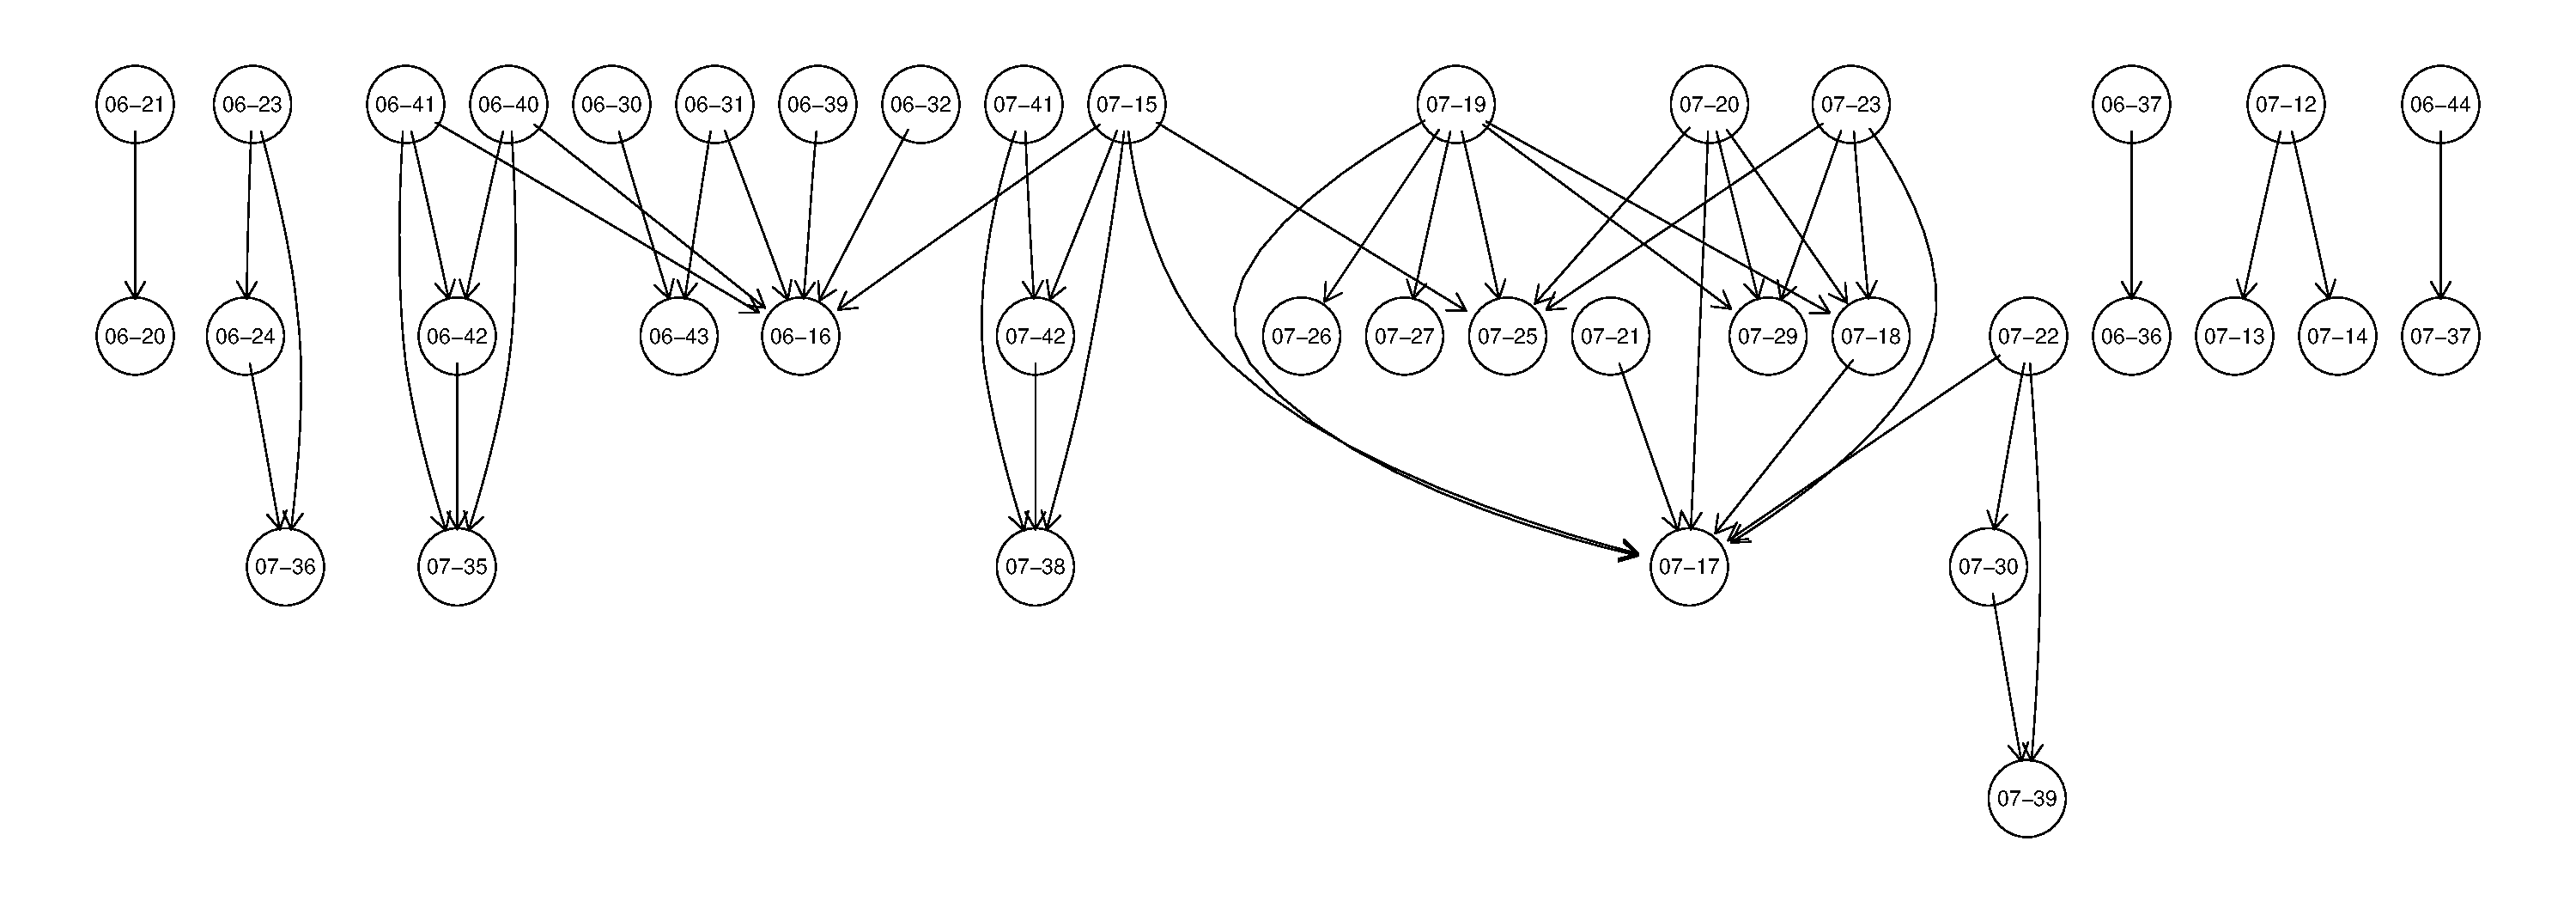
\includegraphics[width=\linewidth]{img/salinet} 
  \caption{A SALI network constructed from XXX. See Ref.~\cite{Guha:2008aa} for further details.}
  \label{fig:salinet}
\end{figure}

Network similarity graphs (NSG's) are an alternative network
visualization of SAR data described by Wawer et al \cite{Wawer:2008aa}
that employs a different characterization of activity cliffs. This
approach is designed to multiplex information by combining
connectivity (representing similarity relationships) with node color
(potency) and size (discontinuity score \cite{Peltason:2007aa}). This
approach has been implemented in the SARANEA tool
\cite{Lounkine:2010fk} and extended \cite{Iyer:2011ij} the NSG concept
to include mechanism of action information.

Networks have been applied to a number of other SAR related
problems. For example, Webb et al \cite{Webb:2014tp} proposed a
network approach to the interpretation of arbitrary machine learning
models. Hanser et al \cite{Hanser:2014gl} constructed a network model
to represent SAR knowledge data, resulting in a ``hypothesis
network''. A key feature of this approach is the ability to integrate
disparate data types and build predictive models on top of the
network. Krein and Sukumar \cite{Krein:2011tt} describe an analysis of
chemical spaces using a graph representation and compare chemical
spaces using network metrics.

\subsection{Assay networks}
\label{sec:assay-networks}

Most high throughput screening campaigns tend to involve multiple
assays. These usually include a primary screen followed by one or more
secondary screens as well as counter-screens. When data from such
campaigns are deposited into public databases such as Pubchem, the
temporal sequence of the assays is not always maintained. As a result
it can be difficult to track the progression of chemical matter
through the series of assays. In addition, a view of the complete
assay sequence can allow one to detect commonalities between programs
and better compare the performance of screening workflows. Calhoun et
al \cite{Calhoun:2012uq} describe an approach to reconstructing
screening workflows (also termed workflow graphs) from screening
datasets. They employed four heuristic rules to construct graphs from
the data as well as using Pubchem Bioassay meta data and text mining
to identify assays from a given project. These assay networks can be
visualized using an online tool located at
\href{http://swami.wustl.edu/flow}{http://swami.wustl.edu/flow}.
Swamidass et al \cite{Swamidass:2014vn} describe an approach to
constructing ``assay networks'' based on Pubchem data, where assays
are connected when they exhibit common active (non-promiscuous)
compounds. In this approach connected assays are correlated since they
exhibit compounds with similar activities. This method leads to
connections between apparently unrelated screen allowing one to
identify compounds that exhibit polypharmacological behavior (i.e.,
activity against multiple targets) and thus are candidates for
repurposing. By also labeling screens as phenotypic or biochemical,
this approach allows one to propose target candidates based on
connectivity, thus serving as one approach to target deconvolution.

\subsection{Scaffold networks}
\label{sec:scaffold-networks}

The notion of a scaffold is common place in medicinal chemistry and is
usually considered to be a ring-containing substructure pruned of
sidechains that represents the core structure of a series of
molecules. An example is the tricyclic core common to a number of
antidepressants (e.g., amitriptylene and imipramine) shown in Figure
\ref{fig:tca-core}. Scaffolds allow one to summarize a collection of
molecules (such as in patent claims) and one can usually assume that
compounds with the same scaffold will share a common synthetic pathway
or even a common mechanism of action.
\begin{figure}[h]
  \centering
  \includegraphics{img/tca-core}
  \caption{An example of a scaffold. In this case, this
  scaffold is common to many tricyclic antidepressants.}
  \label{fig:tca-core}
\end{figure}


While a number of approaches have been described to generate scaffolds
\cite{Lewell:1998aa,Bemis:1996aa,Katritzky:2000wf}, a few approaches
have considered hierarchical decomposition of scaffolds. Examples
include the HierS method \cite{Wilkens:2005il} and the Scaffold Tree
method \cite{Schuffenhauer:2007oz}. The latter generates a series of
scaffolds based on an iterative removal of rings. The output of this
method is a series of scaffolds arranged in a tree-like structure
whose root node represents the simplest ring obtainable from the
starting scaffold.  Two scaffolds are connected if there exists a
parent--child relationship between the two. Scaffold trees generated
by this method lend themselves naturally to network
visualizations. Scaffold Hunter \cite{Wetzel:2009uq} is an example of
a tool that employs a network representation of scaffold trees. Figure
\ref{fig:scafftree} shows an example of a scaffold tree generated from
a set of 602 pyruvate kinase inhibitors. The graph is colored based on
$\log AC_{50}$ and the data is obtained from Pubchem AID 361. This
visualization lends itself naturally to adding overlays such as
molecular properties either on leaf nodes or else as aggregated values
on non-leaf nodes. The scaffold tree has been applied in a number of
studies \cite{Wetzel:2009uq,Renner:2009wm} and the structure of the
tree can be used as a guide to exploring chemical space, focusing on
regions (as represented by a scaffold) where there is minimal activity
(a ``biological hole'') or high activity.

\begin{figure}[h]
  \centering
  \includegraphics[width=0.9\linewidth]{img/scafftree-full}
  \caption{An example of a scaffold tree displayed as a  radial
    network, generated from a set of pyruvate kinase inhibitors.}
  \label{fig:scafftree}
\end{figure}

Varin et al \cite{Varin:2011ve} describe ``scaffold networks'' which
are similar in nature to scaffold trees but instead of a tree
structure where each scaffold has a single parent, a DAG is
constructed by considering all scaffolds at a given level of the
hierarchy. An example of a scaffold network generated from Alosetron
is shown in Figure \ref{fig:scaffnet}, where the blue structures are
those that would be generated using the Scaffold Tree algorithm and
the green structures would be the extra scaffolds generated using the
Scaffold Network algorithm. Using this approach, together with the
compound set enrichment method \cite{Varin:2010zh} the authors were
able to efficiently identify active scaffold and active molecules

\begin{figure}[h]
  \centering
  \includegraphics[width=0.75\linewidth]{img/scaffold-network}
  \caption{An example of the scaffolds generated using
  the Scaffold Tree and Scaffold Network algorithms, starting from
  Alosetron. Blue scaffolds are generated by both methods and green
  scaffolds are generated only by the Scaffold Network
  method. Modified from Figure 1 in Varin et al \cite{Varin:2011ve}.}
  \label{fig:scaffnet}
\end{figure}

\subsection{Scaffold-document networks}
\label{sec:scaff-docum-netw}

With the advent of SAR databases such as ChEMBL \cite{Gaulton:2012jl},
it is feasible to explore chemical space from a bibliometric point of
view. For example, ChEMBL has identified small molecules mentioned in
publications and provides the links between them. As a result, given a
set of document it is possible to characterize the chemical space
represented in those documents. As noted in Section
\ref{sec:scaffold-networks}, scaffolds (or frameworks) allow one to
better capture the core structures representing multiple
compounds. Thus, a publication might refer to ten compounds from a
single series, in which case it refers to a single scaffold (though
this could depend on how one defines a scaffold). To explore this
aspect of a SAR database, we applied a fragment decomposition method
to all compounds reported in ChEMBL and linked the fragments
associated with each molecule to their corresponding documents. The
resultant data can then be represented as a bipartite network of
fragments and documents which are connected when a document contains
molecules that have the fragment as a substructure. 

One application of this dataset is to explore the nature of fragments
associated with a document, and for each of those fragments identify
the documents associated with them. This procedure can be repeated to
construct scaffold-document network that represents the chemical and
bibliometric space associated with a starting document. As an example
of this type of analysis we constructed a network starting from a
report describing a series of imidazonaphthalimides and their
antitumor activity \cite{Brana:2002pr}. The network was limited to 3
iterations (document $\rightarrow$ fragment $\rightarrow$ document
$\rightarrow$ fragment). In addition we applied constraints on the
fragments (e.g., must be contained in 20 to 50 molecules and exhibit a
minimum complexity), resulting in a network with 1277 nodes (816
document nodes and 461 fragment nodes) shown in Figure
\ref{fig:scafodcnet}. 
\begin{figure}[h]
  \centering
  \includegraphics[width=\linewidth]{img/12477366}
  \caption{An example of a scaffold-document network, limited to three
    iterations. Squares represent fragments and circles represent
    documents. Document nodes are colored based on their major topic
    MeSH heading. The seed document is shown with a red border (top
    left).}
  \label{fig:scafdocnet}
\end{figure}
In this figure, fragment nodes are squares and document nodes are
circles, colored by the major topic MeSH heading. (Only the 12 most
frequent MeSH headings are considered - document nodes outside this
set are colored grey). Though difficult to navigate as a static  
figure, the network structure is interesting in that the immediate
neighborhood of the seed document (red border, top left) is relatively
small. The median number of fragments associated with a document is 1,
(though two documents were connected to more than 100
fragments). Conversely, the median number of documents connected to a
fragment was 3. Fragments tend to be associated with multiple
documents (which is expected based on the number of iterations used to
construct the network, as well as the constraints on fragment
characteristics) and based on the MeSH headings there is topical
overlap between many of these documents. For example, most document
clusters are annotated with the \emph{Chemistry} and \emph{Chemical
  synthesis} MeSH headings. Given that the seed document has been
annotated with \emph{Chemical synthesis} it is not surprising that
based on the chemistry contained within it, related documents will
also be related to synthesis. Importantly, if one considers all
documents in ChEMBL (with valid Pubmed ID's), the two most frequent
MeSH headings are \emph{Chemistry} and \emph{Chemical synthesis} and
thus overrepresentation of these terms is unsurprising. 

This discussion has focused on the document nodes in this network. One
could also examine the fragment nodes, in terms of their similarity to
each other. Alternatively, one could examine the ``history'' of a
fragment in terms of its representation in publications over
time. Since ChEMBL also provides bioactivity data for the compounds in
a document this network representation could be used to track the
progression of bioactivity of a scaffold (or rather its members) over
time.




\section{R as a Platform for Network Analyses in Drug Discovery}
\label{sec:r-as-platform}

The core concepts involved in computational drug discovery can be
reduced to genes, proteins, pathways and small molecules interacting
with them. Computational representations of these concepts and the
methods to be manipulate them have been implemented in a variety of
software tools. A comprehensive computational drug discovery platform
will include a number of these tools, as it is rare that a single tool
addresses all aspects.

In this sense, the R environment presents a robust platform for
computational drug discovery, especially the stages up to and
including lead optimization. The Bioconductor set of packages provide
a plethora of tools to analyze a variety of ``omics'' data. Examples
include packages that support gene expression (microarray or RNAseq)
analyses, tools for differential expression analysis, gene and pathway
enrichment analysis and so on. 

In contrast, support for small molecule data is limited. Currently,
there are two packages that focus on representing and manipulating
chemical structures - \texttt{ChemmineR} \cite{Cao:2008fj} and \rcdk
\cite{Guha:2007aa}. Both expose cheminformatics functionality
implemented in an underlying Java library (JOELib for ChemmineR and
the CDK for \rcdk). In this section we focus on the use of \rcdk as a
means to manipulate and analyze chemical structure data.

The \rcdk package supports a variety of chemical structure file
formats and presents the CDK Java API as a set of idiomatic R
functions. That is, rather than manually specify fully qualified Java
packages or resort to writing ``Java in R'' the \rcdk package wraps
much of the CDK API as ordinary R functions. Thus the atoms in a
molecule are represented as a set of atom objects. Importantly, atoms
(and other objects such as bonds and molecules) are stored as
references to Java objects. While they can be manipulated directly, it
is unwieldy it is recommended that one uses methods provided by the
\rcdk package.

For a detailed review of \rcdk functionality, the reader is referred
to Guha \cite{Guha:2007aa}. For now we focus on simple network
analyses that involve chemical structures. Given a set of compounds
represented as SMILES strings, \rcdk can be used to parse them,
compute binary fingerprints and then compute a pairwise Tanimoto
similarity matrix, as shown below
\begin{lstlisting}
library(rcdk)
library(fingerprint)

mols <- parse.smiles(mipe$SMILES_STD)
fps <- lapply(mols, get.fingerprint, type='extended')
fpsim <- fp.sim.matrix(fps)
colnames(fpsim) <- mipe$SAMPLE_NAME
rownames(fpsim) <- mipe$SAMPLE_NAME
fpsim[ fpsim < 0.6 ] <- 0
\end{lstlisting}
In this code snippet, we compute a pairwise similarity matrix that we
will eventually use as an adjacency matrix to construct the similarity
network. We only keep those similarity values greater than 0.6 so as
to focus only on similar molecules. 

\begin{figure}[h]
  \centering
  \includegraphics[width=\linewidth]{img/sim-network-connected}
  \caption{An example of a similarity network, where nodes are
    molecules and are connected if they exhibit a Tanimoto similarity
    greater than 0.6. Nodes are colored based on the PANTHER
    \cite{Mi:2005qq} class of their primary target.}
  \label{fig:simnet}
\end{figure}

The resultant similarity matrix can be treated as an adjacency matrix
and used as input to \igraph and subsequently plotted
\begin{lstlisting}
g <- graph.adjacency(fpsim, mode='undirected', 
                     weight=TRUE, diag=FALSE)
plot(g, layout=layout.fruchterman.reingold)
\end{lstlisting}
As example of such an analysis is shown in Figure \ref{fig:simnet}. In
this network, we consider a set of 1,341 compounds annotated with a
primary gene target. For each target, the highest level PANTHER
\cite{Mi:2005qq} classification was determined and used to color the
nodes. In addition, we ignore compounds that were less than 0.6
similar to any other compound (i.e., singleton nodes).

This is purely a visualization of a similarity matrix,
modified to focus on similar (according to a specified threshold)
compounds. Importantly, we have been to overlay a second type of
information (i.e., target class) on top of the similarity values and
is thus an example of the integrative nature of a network
representation.

Given the compound network and the associated target information, one
could easily identify protein-protein interactions (BioGRID
\cite{Chatr-Aryamontri:2015yf}, STRING \cite{Franceschini:2013qa} and
other sources) and generate a bipartite graph of compounds and protein
targets. Even in the trivial, annotated network show in Figure
\ref{fig:simnet} it is evident that chemical similarity is related to
functional similarity of the compounds' primary target - compounds
targeting cytoskeletal proteins tend to be similar to each other;
though interestingly, within the set of compounds targeting
cytoskeletal proteins there appear to be five distinct groupings. When
coupled to an interactive platform, this visualization can support
rapid identification and exploration of novel associations.

% While the \rcdk package and its dependencies provide general small
% molecule handling functionality, a number of other packages provide
% more specific functionality, related to small molecules. We have
% previously mentioned DrugComboRanker \cite{huang2014drugcomboranker}
% and MANTRA \cite{iorio2010discovery}.

\section{Discussion}
\label{sec:summary}

In this chapter we have attempted to provide an overview of how
networks have been employed to analyze and visualize chemical
data. The fact that chemical structures themselves are graphs allows
one to apply a number of techniques from graph theory to characterize
chemical structure (such as the many graph invariants). However, with
the advent of large collections of chemical structures (from databases
such as Pubchem or high throughput screening programs) along with
associated data such as bioactivity and target annotations, a number
of workers have attempted to analyze the properties of such
collections using network techniques.

It is interesting to note that many applications of network methods to
chemical collections focus on visualization of the chemical data,
rather than using the network structure to draw insight into the
underlying chemical of biological phenomena. This is not to say that
network visualizations of chemical data are lacking. In fact, such
visualizations allow one to encode multiple properties of objects
(i.e., nodes) and relationships (i.e., edges) in a single visual form. 

However, a key utility of network approaches is the ability to
integrate different data types (such as small molecules and their
protein targets) in to a single data structure. Drug-target or
drug-disease (or even drug-disease-target) networks are examples of
such approaches. Hartsperger et al \cite{Hartsperger:2010yg} describe
an approach to fuzzy clustering that is capable of identifying
subgraphs with heterogenous networks. A characteristic feature of such
$k$-partite networks is that it allows one to model the effects of
each class of entity on other classes of entities. This is exemplified
by random walk approaches on bipartite networks such as that described
by Chen et al \cite{Chen:2012qy} whose proposed a random walk approach
to predict drug-target interactions.

\bibliography{paper}

\end{document}
